Since the project was done as a double-period course at \LTU, $\SI{400}{\hour}$ per person was planned for the project over four months, this would amount to $400\cdot15=\SI{6000}{\hour}$ in total. To plan these hours, an agile workflow was adopted by dividing the work into sprints of two weeks each, where the end of each sprint represented a project presentation.

Each presentation required some new features to be displayed, so goals representing those features were made up at the very start of the sprint and added to the taskboard. The developers then visited the taskboard to assign themselves new tasks that they believed they could handle and started working on it.

For instance, in the first presentation the architecture was to be presented and a simpler technical demonstration was planned. So, a proof-of-concept wherein python code was to be tested using a very simple user interface was designed. The idea was to include some mock data from the backend as well, but at the day of the presentation, the API was not yet ready. Therefore, right after the presentation, a new sprint goal to have the database setup and storing the progress of the corrected tests was planned for the next week.

\subsection{Milestones}
During the planning of the project some milestones were established to keep track of the progress toward the end-product. A milestone describes a major goal in the development, such as major steps of the pre-study and the introduction of new features to the system. Aside from the initial milestones additional goals emerged during the pre-study and development. The identified milestones are described briefly below in the approximate order they were planned to be realized.

\subsubsection{Gamification research}
In order to identify gamification elements suitable for the system research in the subject was to be conducted.

\subsubsection{Interviews}
As the system to be developed was planned to be deployable for programming courses at LTU interviews with teachers were planned in order to identify use-cases.

\subsubsection{Workshop}
A workshop where educators were to be invited was planned. Scenarios were to be presented to promote discussions around how courses could be made interesting to students, and easy to maintain as a teacher. A detailed description of the scenarios can be found in appendix \ref{sec:workshop}.

\subsubsection{Code testing}
A core feature required for the basic functionality of the system is the ability to run tests on submitted code. For this purpose some sort of tester service needed to be created.

\subsubsection{Backend server running}
A basic backend server that would eventually manage a database and serve data to a frontend needed to be developed.

\subsubsection{Frontend server running}
A basic frontend server that would eventually visualize the system by serving HTTP data to clients needed to be developed.

\subsubsection{Connect entire architecture}
A major milestone would be to connect the entire architecture. This consists of being able to send requests to basic backend routes from the frontend, by doing so modifying the database, and submit code to the tester and retrieve a result.

\subsubsection{Tester scalability}
The tester needs to scale well with increased load, so a good way of allocating resources needed to be put in place.

\subsubsection{Login with CAS}
Since the target users of the systems are students and educators using CAS for authentication was deemed suitable. This would also remove the need for the system to handle passwords.

\subsubsection{Complete backend API}
The set of backend routes needed to modify the essential database collections needed to be completed.

\subsubsection{Working game elements}
The game elements that were decided upon in the pre-study needed to be implemented.

\subsubsection{Course invites}
The ability for teachers to invite students to courses needed to be implemented.

\subsubsection{Statistics}
A feature for teachers to view statistics, such as assignment completion rates for courese, needed to be implemented.

\subsubsection{Multi-player}
It was decided that multi-player features such as group assignments could be useful for increasing motivation in learning.

\subsubsection{Additional login providers}
For the system to be deployed at other locations than LTU additional login providers need to be supported.

\subsection{Taiga Sprint Planner}
Sprint planning was done using the open-source \taiga{} taskboard. By using a web-based tool, most planning could be done remotely instead of on a physical whiteboard. An idea was that it would allow participants to do their work remotely and not have to bother with visiting the project room. Taiga was chosen because it offered a free and gratis environment with little hassle for public projects, which seemed like a good fit for this project since everyone was eager to get started.

\begin{figure}[hb]
    \begin{subfigure}{.3\textwidth}
        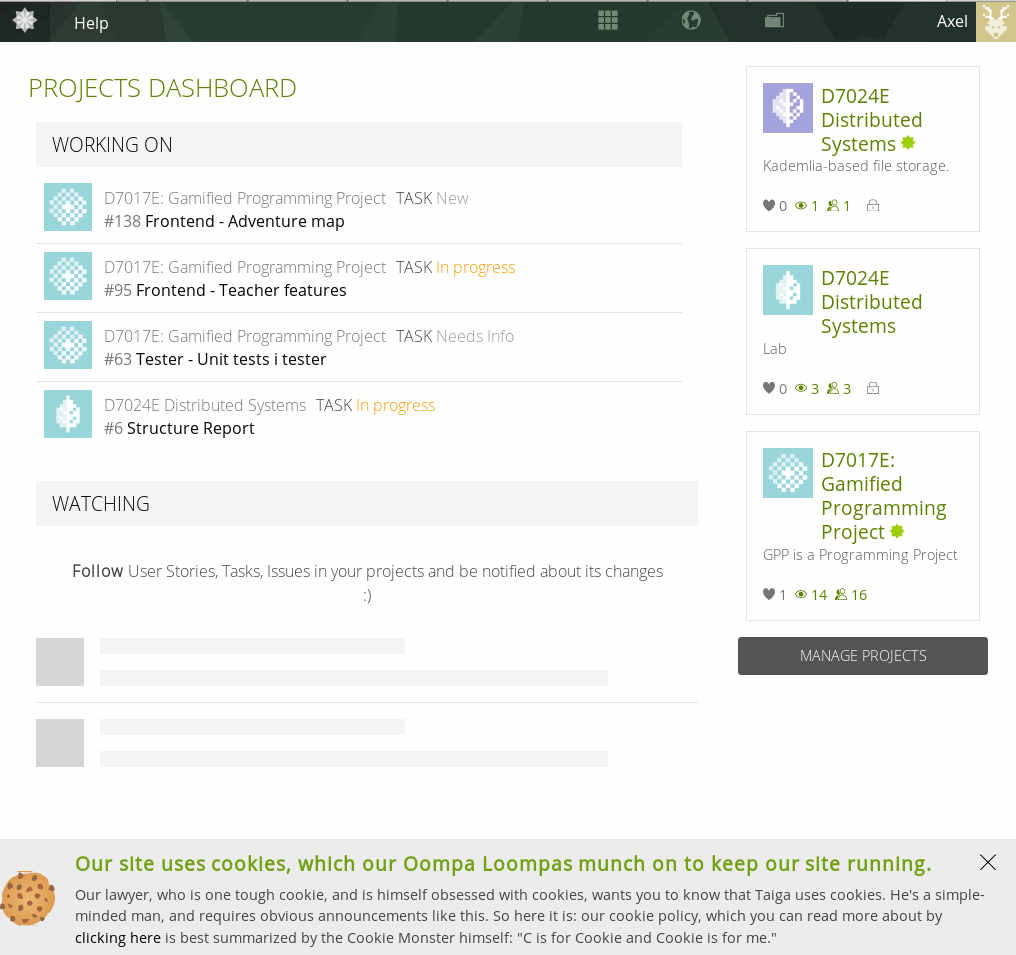
\includegraphics[width=\textwidth]{img/taiga_dash.jpg}
        \caption{Main dashboard}
    \end{subfigure}
    \hfill
    \begin{subfigure}{.3\textwidth}
        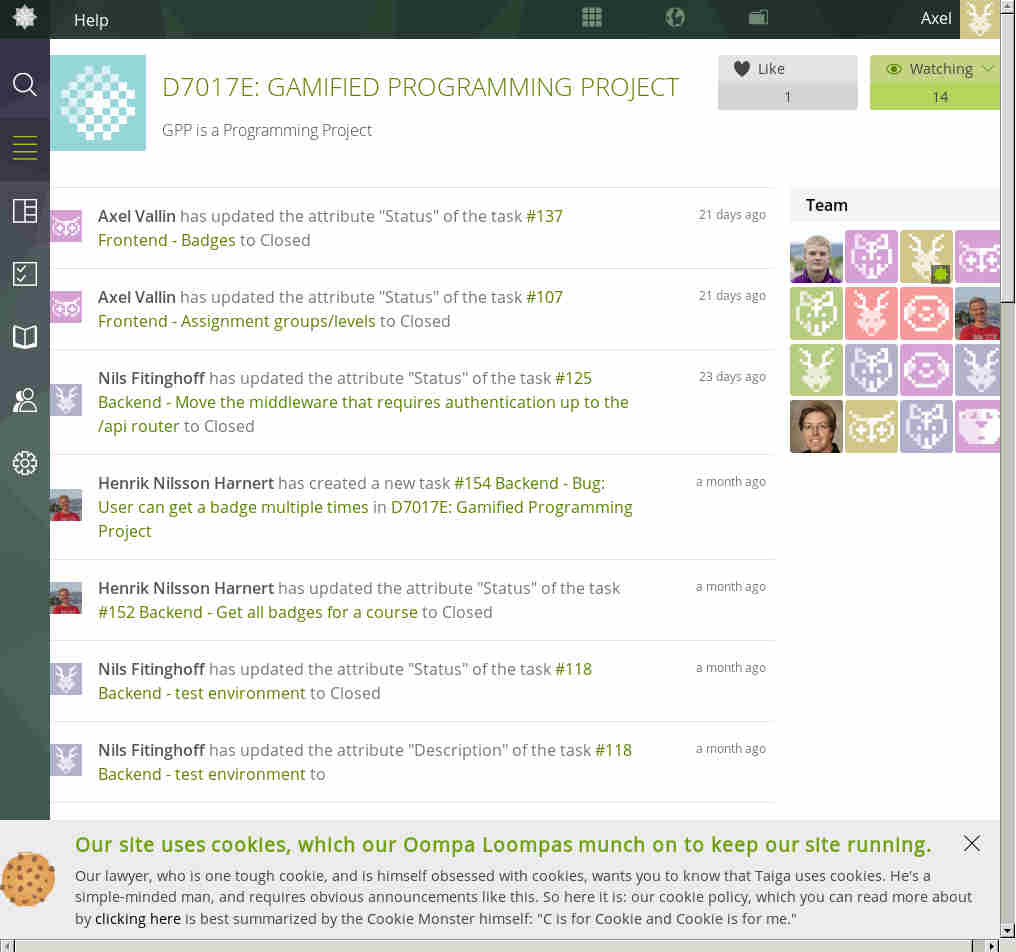
\includegraphics[width=\textwidth]{img/taiga_overview.jpg}
        \caption{Overview}
    \end{subfigure}
    \hfill
    \begin{subfigure}{.3\textwidth}
        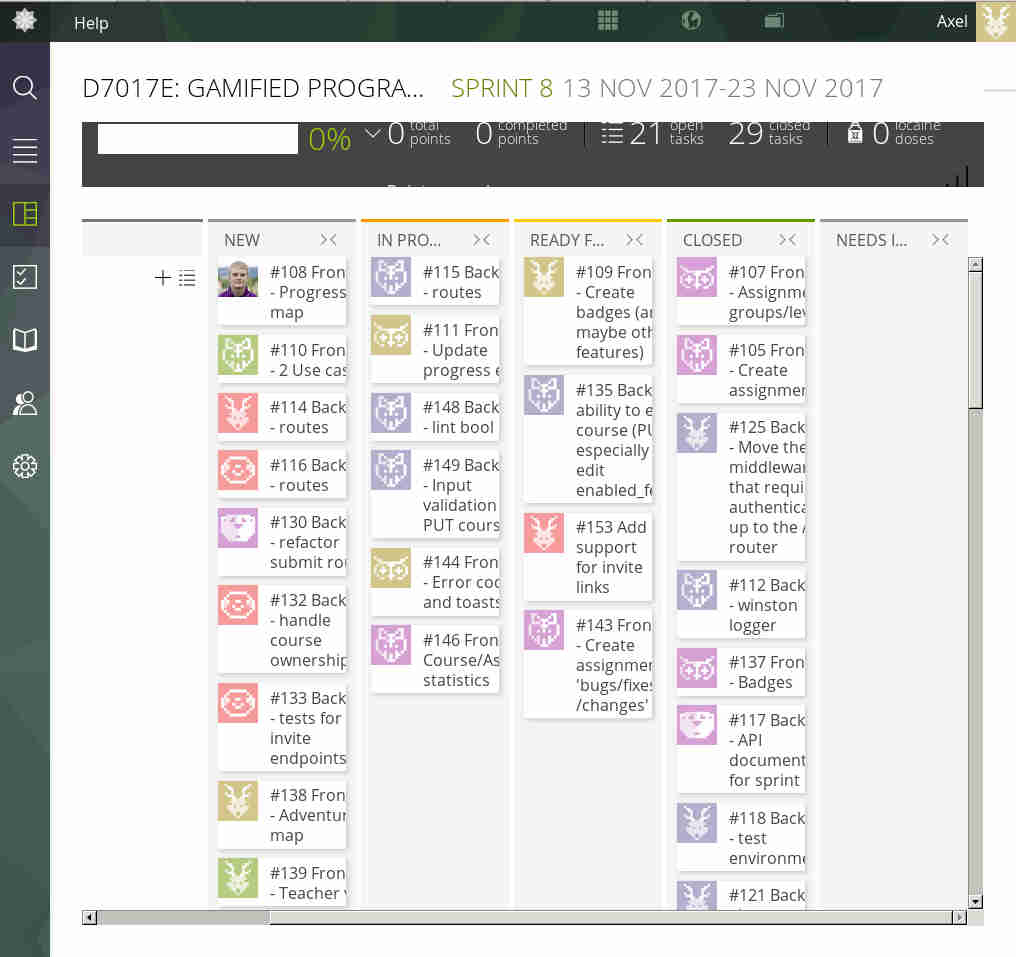
\includegraphics[width=\textwidth]{img/taiga_taskboard.jpg}
        \caption{Taskboard}
    \end{subfigure}
    \caption{Some screenshots from \taiga{}.}
\end{figure}

%Apart from \taiga{}, Trello was evaluated, but deemed too simple for a project of this size, furthermore some pay-to-use tools such as TODO: was looked at, but nobody wanted to pay for the service.
